
\section{Casing}
This system has some different types of components and sensors, which all need to be housed in a watertight casing for security and robustness. Some design ideas for this part was to make it easy to mount, small physical footprint, all the electronics in the same enclosure and watertight.  

The case will be revised and worked on over the whole length of the course, redefining and remodeling the construction over time.  

The cases are constructed with the use of the program Fusion 360, which is a free to use CAD software. They are then produced by using a 3D printer, which is a fast and easy way of try out different ideas and models.   

%% Första versionen -------------------------
\subsection{First revision}
First, a suitable solution was needed, with no thoughts about physical limitations, strength, material or manufacturability.  

The idea was modeled around the original mounting plate which is already fastened to the boat, which has the function to hold the board in place and make the daggerboard stable in the boat. The model had the same dimension as the original plate, only the height was different to accommodate the size of the pressure sensors. By making a mounting plate with the same width and length of the original mounting plate the implementation would be neat and space saving. 

This one had some problems, one of them is that the case is too big for any of the 3D-printers that we had access to. Another problem with this instance of the model was that for the circuit boards to fit inside they had to be very small and have some odd shapes.  

% Kolla på mina bilder


\begin{figure}[H]
\begin{center}
	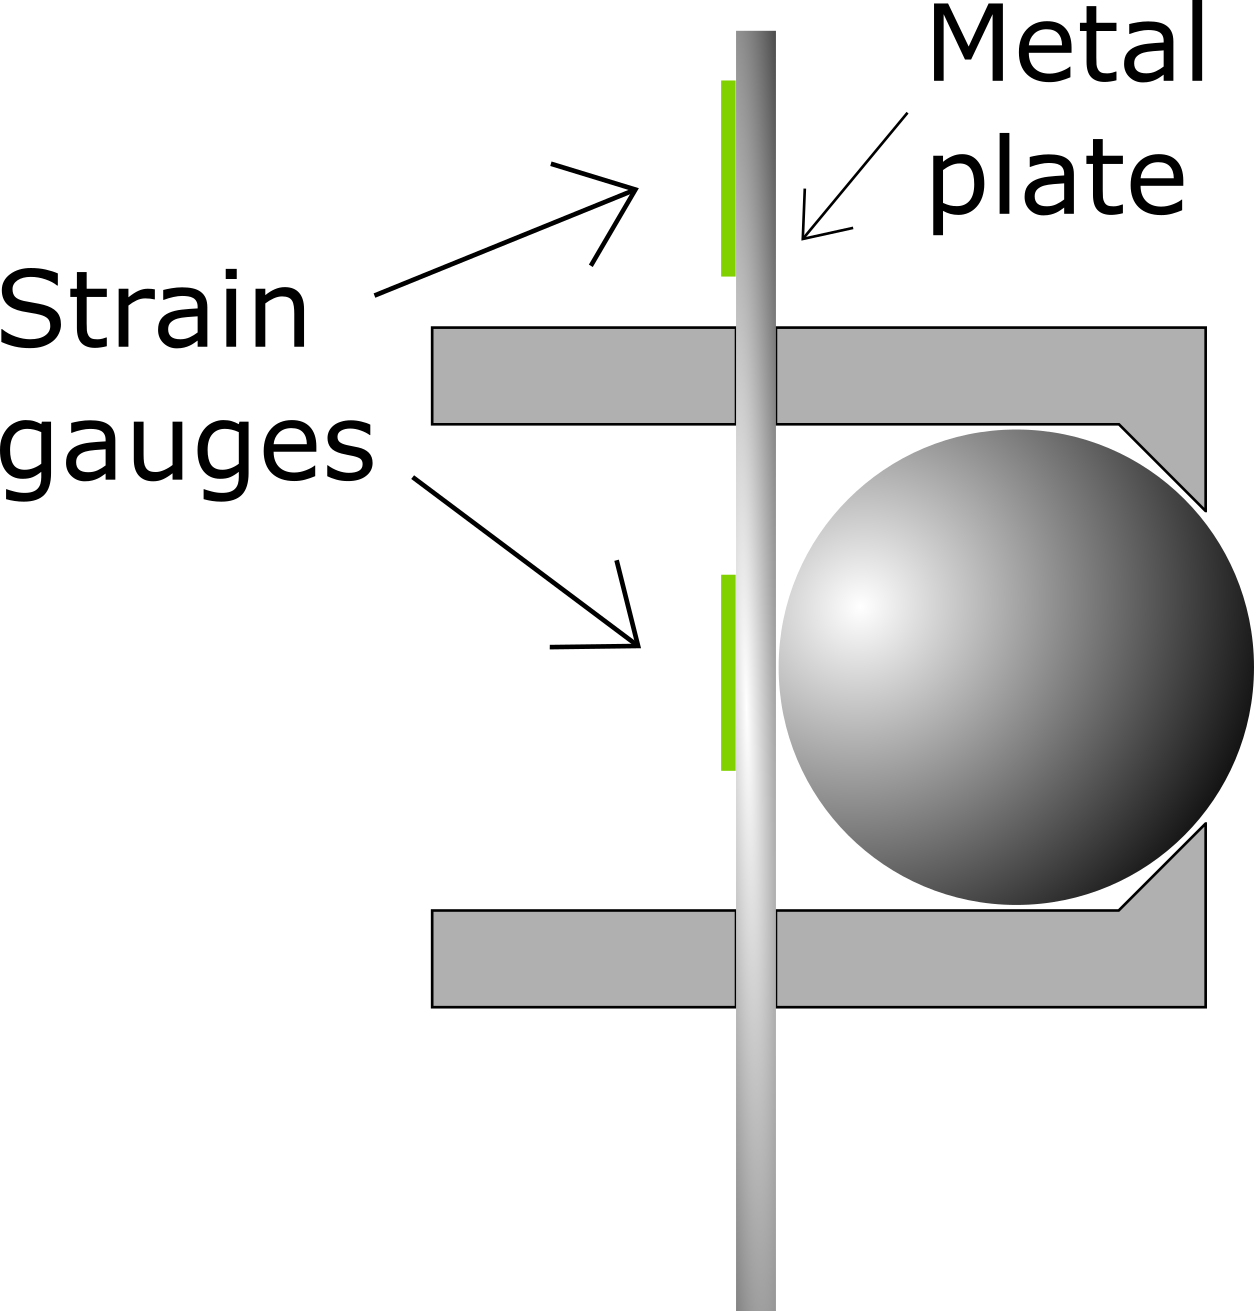
\includegraphics[width = 10cm]{Figures/Press_sens_func_1.png}
	\caption{Function of first prototype}
	\label{Press_sens_prot_1}
\end{center}
\end{figure}

%% Andra versionen -------------------------
\subsection{Second revision}
The next revision was like the first one, it had the same shape and idea as the first one by having the same size as the original plate, but this time it only consisted of the front part that holds the sensors and all the electronics. This version can thus be made on a 3D-printer. It still has the problem of having very little space for all the components.    

% Kolla på mina bilder
\begin{figure}[H]
\begin{center}
	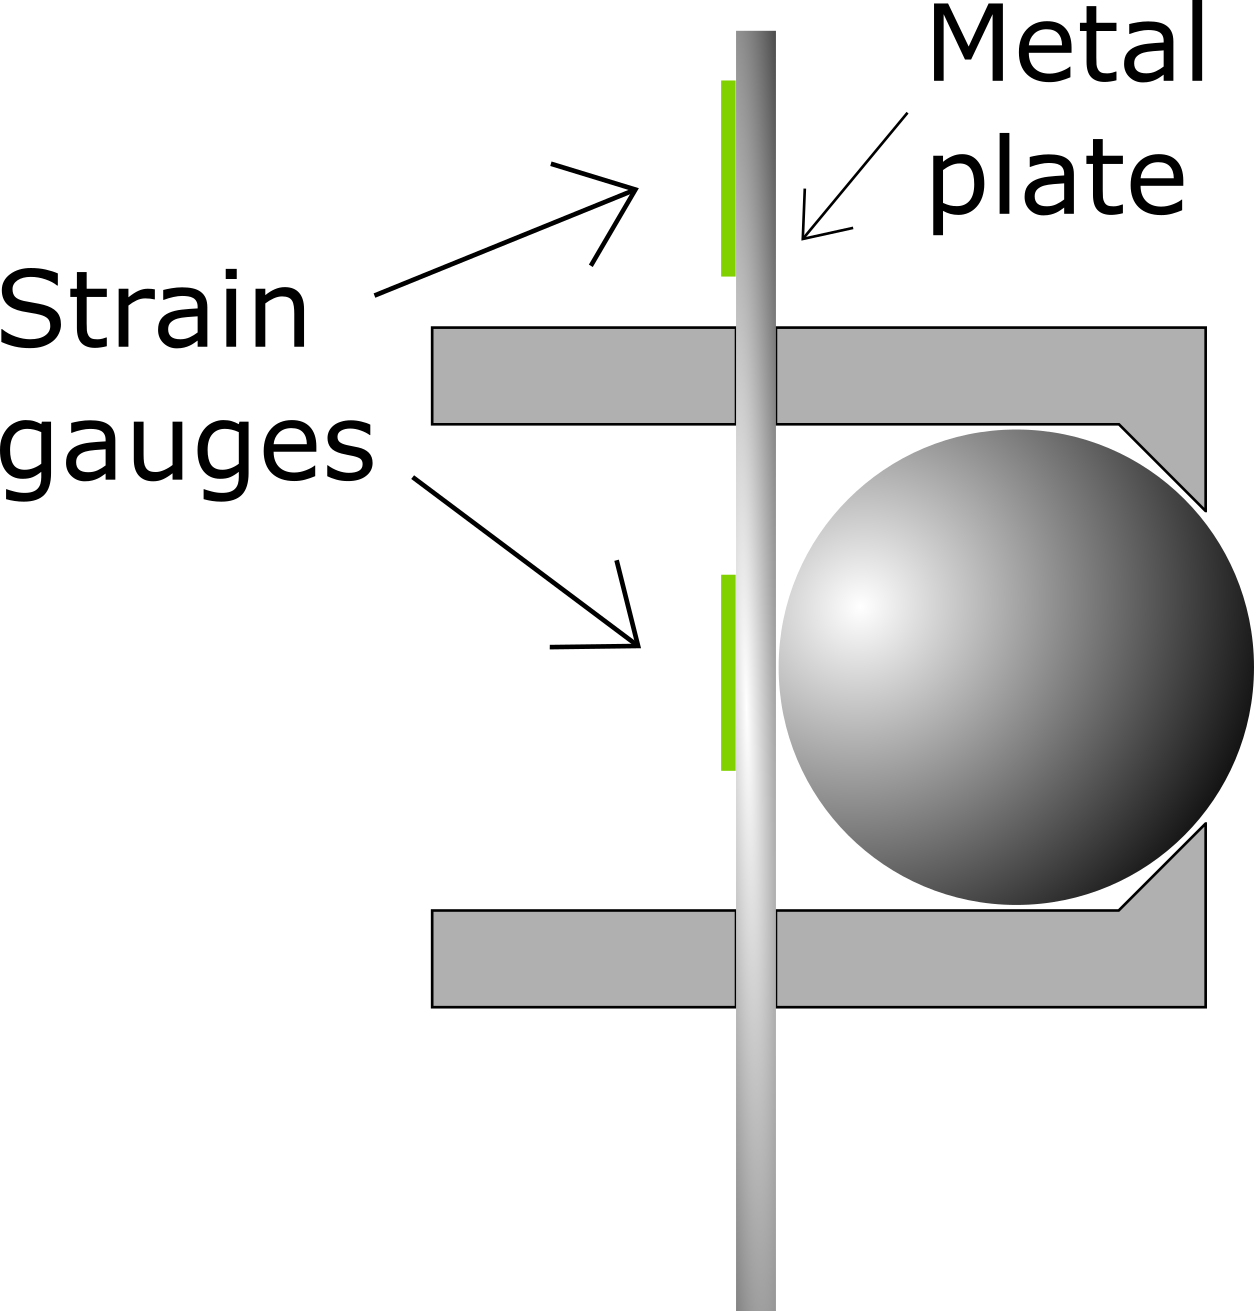
\includegraphics[width = 10cm]{Figures/Press_sens_func_1.png}
	\caption{Function of first prototype}
	\label{Press_sens_prot_1}
\end{center}
\end{figure}

%% Tredje versionen -------------------------
\subsection{Third revision}
With all the prior knowledge, the next version was modeled. This time it had a much larger casing to accommodate for the PCB. The actual size of the PCB was set by the inner dimensions of this part.  

This case still had some problems, it did neither include a holder for the distance sensor nor being watertight. But this version was also good in many aspects. The size of the part was enough to accommodate for the PCB, batteries and all the sensors.  

This part was created using a 3D-printer to have some progress to show, check for design faults and to determine improvements for the next version.  

Due to the fundamental workings of a 3D-printer the size and dimension on the real produced part differed some from the CAD model. When construction with a 3D-printer the model needs to be compensated for this. One thing that needed to be revised was the implementation of the steel beads.  

When building the third version on the 3D-printer the problems with the model could be more easily determined than only looking at a design in a CAD software. The process of improving the design is both about the physical limitations and the issues  due to the manufacturing process. 

% Kolla på mina bilder

\begin{figure}[H]
\begin{center}
	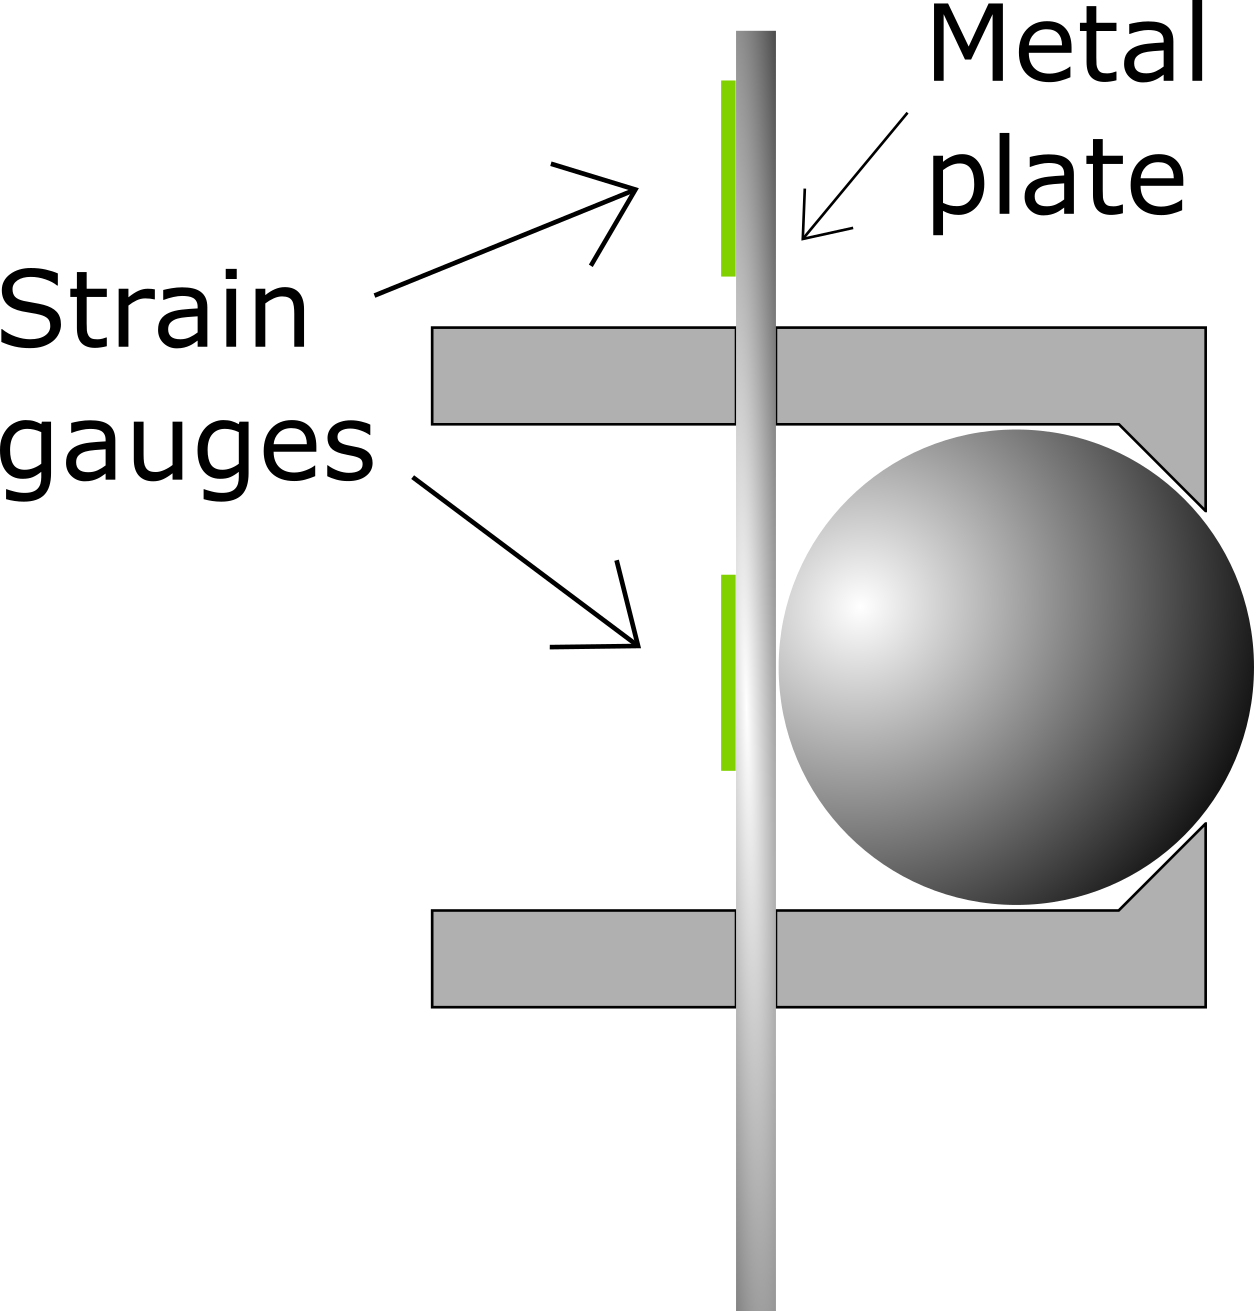
\includegraphics[width = 10cm]{Figures/Press_sens_func_1.png}
	\caption{Function of first prototype}
	\label{Press_sens_prot_1}
\end{center}
\end{figure}

\subsection{Fourth revision}

The fourth revision has all the features and can hold all the electronics. It's been designed to hold the power switch in the front, the Time of Flight sensor on the top, the load cells, the batteries and both the PCBs in the same enclosure. The access panel has been placed at the underside of the model to get a better water seal. The access panel is a big plate covering the most part of the underside of the model. To ensure it's watertight there is a seal between the panel and the casing itself.
Due to the material cost and time it takes for the 3D printer to produce models the manufactured part has just some thin layers in the bottom part of the print. To get the some strength in the model epoxy resin was mixed and poured in to both get the stability needed and a clear window for the Time of Flight sensor.

\subsection{Results}
The final version is the product of many revised and improved steps. The model holds all the electronics and sensors in the same enclosure and takes up as small physical space as possible. A 3D printer is used to produce the core structure and epoxy resin and some rubber is used to get the stiffness and water tight The final adjustmends made to the model inncludes a mountig solution for the 
Time of Flight sensor, revised implementation of the pressure sensors, modified the PCB mountings, and small changes to 
Problems :
The pressure sensors is not entirely water sealed, some more work is needed in that area.  

\subsubsection{The prototype}

% Kolla på mina bilder
\begin{figure}[H]
\begin{center}
	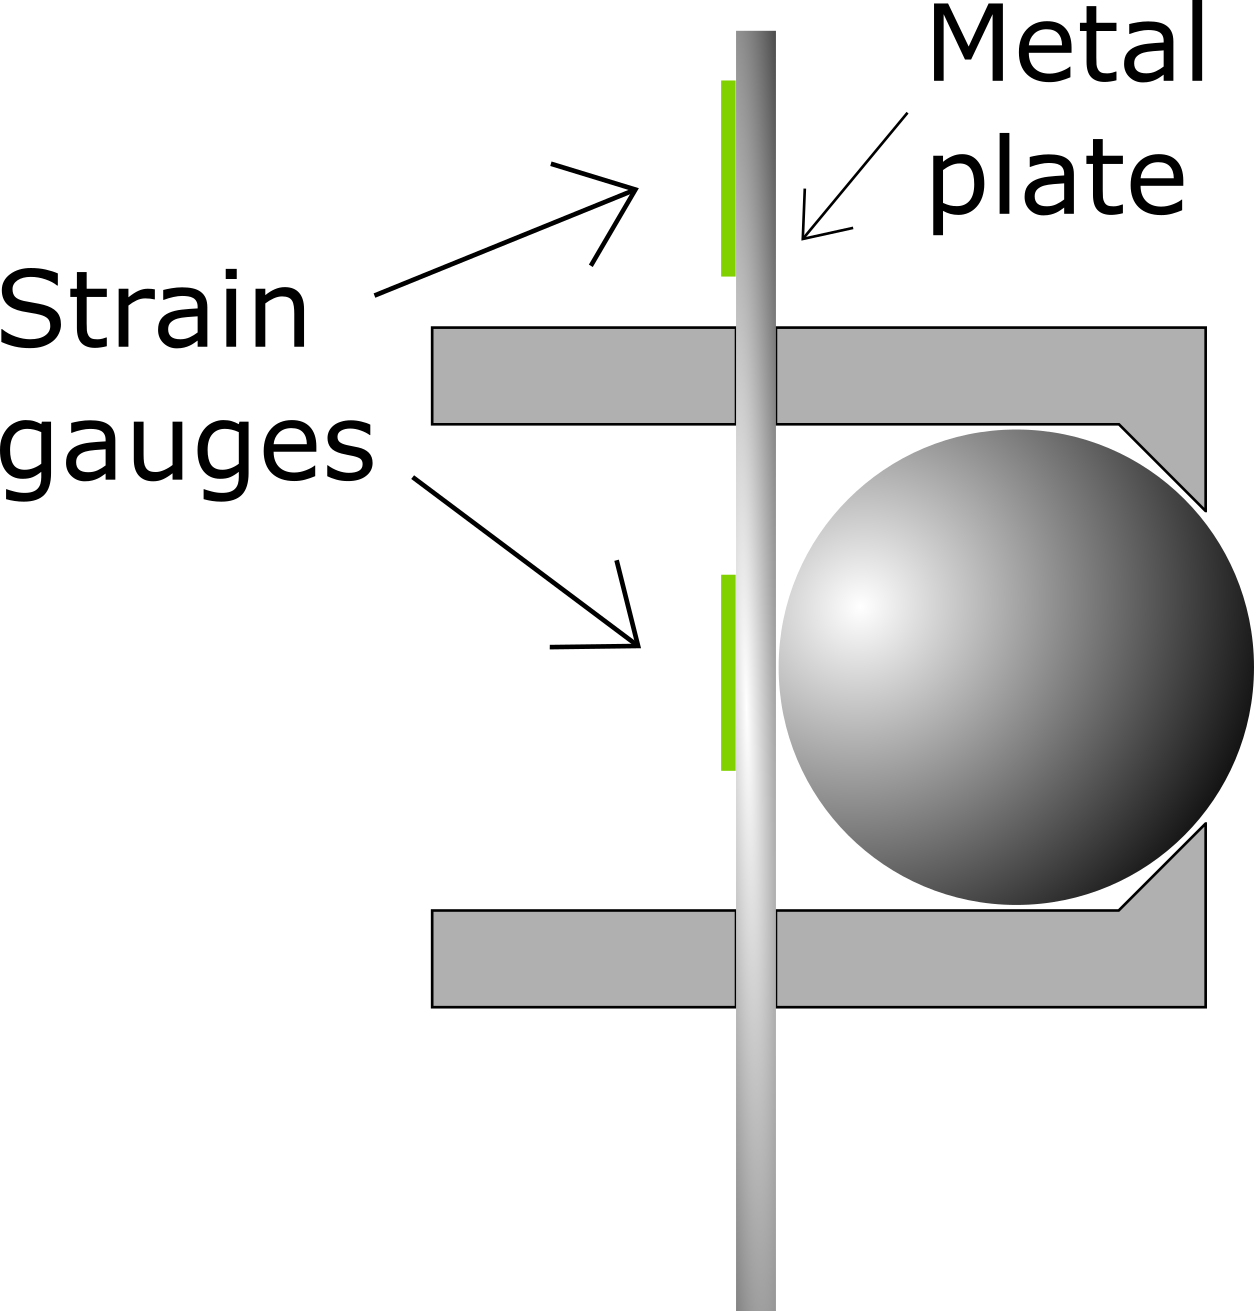
\includegraphics[width = 10cm]{Figures/Press_sens_func_1.png}
	\caption{Function of first prototype}
	\label{Press_sens_prot_1}
\end{center}
\end{figure}
